Nykyisen arkkitehtuurin ongelma ovat useat integroinnin LDAP-palvelimeen. LDAP:in on talletettu jäsenten henkilökohtaista dataa, kuten henkilötunnus, joten tietoturvasyistä siihen halutaan integroida mahdollisimman vähän eri sovelluksia. Tällä hetkellä sovelluksia on vain Sikteeri ja admtool, mutta pidemmän aikavälin tavoitteena on uusien palveluiden (kuten käyttäjien palvelunhallinta) toteuttaminen sekä nykyisen Sikteerin jakaminen pienempiin osapalveluihin palvelusuuntautuneen arkkitehtuurin mukaisesti. Kuvassa \ref{kapsi_uusi} on esitetty tavoiteltu arkkitehtuuri, jossa Sikteerin laskutus- ja jäsenrekisteripalvelut on itsenäisiä web-sovelluksia ja joiden rinnalla on admtool-komentorivityökalu sekä käyttäjien palvelunhallinta. LDAP:n integraatiopisteiden määrä on yksi, sillä LDAP kommunikoi vain keskitetyn tunnistautumispalvelun kanssa, joka taas tarjoaa Kapsi ry:n web-sovelluksille tunnistautumisrajapinnat.

\begin{figure}[ht]
\centering
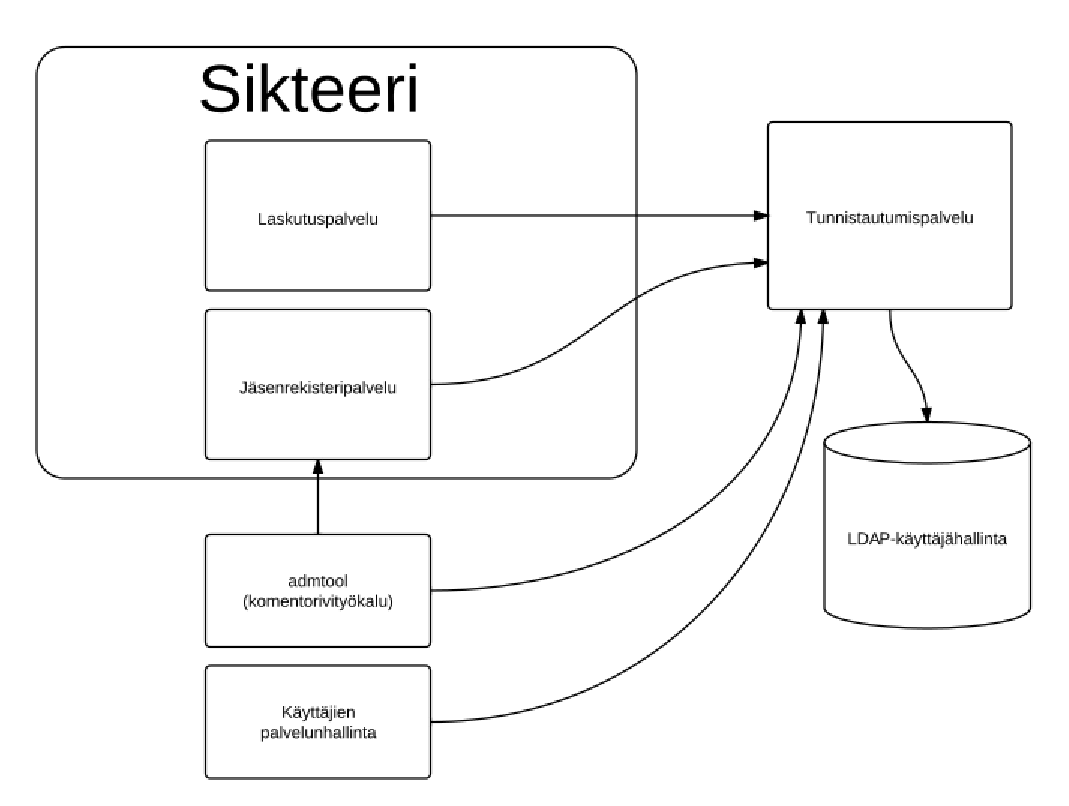
\includegraphics[width=.7\textwidth]{toteutus/kapsi_uusi.eps}
\caption{Palvelusuuntautuneen arkkitehtuurin mukainen kuvaus Kapsin järjestelmästä. Sikteerin palvelut on jaoteltu omiksi komponenteiksi ja järjestelmään on lisätty keskitetty tunnistautumispalvelu.}%
\label{kapsi_uusi}
\end{figure}

Tämän tutkielman kannalta oleellisin osa uudessa arkkitehtuurissa on keskitetyn tunnistautumispalvelun toteuttaminen. Sikteerin nykyinen toteutus ja suunniteltu jatkokehitys asettavat tiettyjä vaatimuksia toteutettavalle tunnistautumispalvelulle. Näitä vaatimuksia sekä muita reunaehtoja käsitellään seuraavassa alaluvussa.

\subsubsection{Vaatimukset ja reunaehdot}
- yleisesti tuettu teknologia, eli käytännössä OAuth, OpenID, SAML... erityisesti python-tuki tärkeää. reunalla voidaan siis olla, kunhan ainakin tuettu python-kirjasto löytyy
- täytyy tukea myös komentorivityökaluja, joten pelkkä user-agent flow ei riitä. Tämä supistanee vaihtoehdot OAuthiin ja SAML:in, OpenID on jotain muuta?
- eri tasoisia käyttäjiä, joten pelkkä autentikoituminen ei riitä, vaan täytyy myös pystyä passaamaan käyttäjän attribuutteja
- koodia halutaan muuttaa mahdollisimman vähän nykyisissä softissa